\documentclass{scrartcl}			% defines the kind of document you want to produce

% Include different packages:
\usepackage[utf8x]{inputenc}
\usepackage[T1]{fontenc}
\usepackage{lmodern}
\usepackage[english]{babel}
\usepackage{amsmath}
\usepackage{graphicx}           	% include graphics
\usepackage{caption}	
\usepackage{subcaption}	 
\usepackage{hyperref}
\usepackage{epstopdf}
\usepackage{siunitx}
\usepackage{float}

\title{Neuroprothetics Exercise 6\\Electric Stimulation}
\author{ Laura Bielenberg }
\date{14. Juni 2019}

\begin{document} 					% Document begins here

\maketitle

\section{Calculate the Potential Field}
The code used to generate the following plots can be found under \texttt{code/exercise\_6.py} and \texttt{code/Neuroprosthetics/potential\_fields.py}.\\
The potential at a distance $r$ from a current point-source can be calculated by:
\begin{equation}
\Phi = \frac{\rho_{medium}\cdot I}{4\cdot\pi\cdot r}
\end{equation}

\subsection{Potential Field}
Figure~\ref{fig:pot_field} shows the plot of a potential field for a $\SI{50}{\micro\meter}$ by $\SI{50}{\micro\meter}$ slice  in a distance of $\SI{10}{\micro\meter}$ from the point source. The used parameters are:
\begin{itemize}
\item $\rho_{medium} = \SI{300}{\ohm\cm}$
\item $I = \SI{1}{\milli\ampere}$
\item $resolution = \SI{1}{\micro\meter}$ 

\end{itemize}

\begin{figure}[H]
\centering
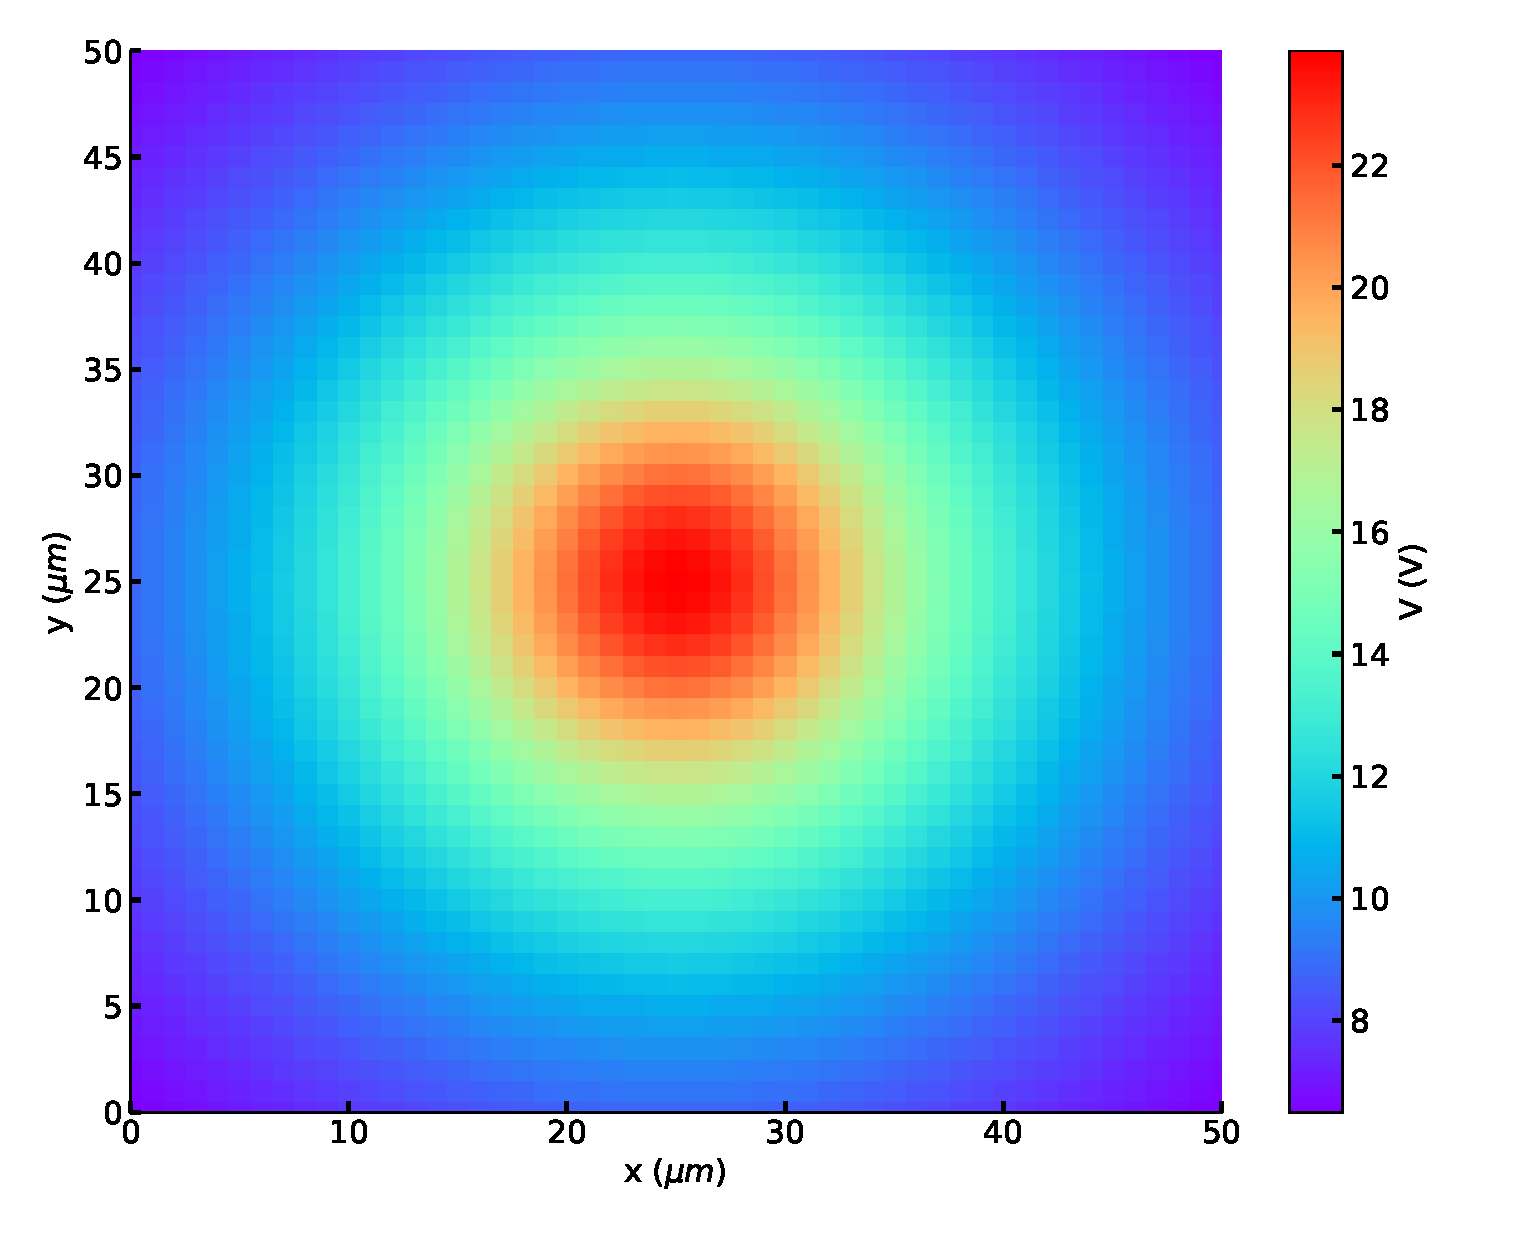
\includegraphics[width=\linewidth]{imgs/potentialfield.eps}
    \caption{Potentialfield for a $\SI{50}{\micro\meter}$ by $\SI{50}{\micro\meter}$ slice in a distance of $\SI{10}{\micro\meter}$ from the point source.} 
    \label{fig:pot_field} 
\end{figure}

\subsection{Activation Function}
Calculate and plot a) the external potential, b) the electric field and c) the activation function along a $\SI{50}{\micro\meter}$ peace of axon positioned $\SI{10}{\micro\meter}$ from a current point source. Plot the three graphs for a electrode current of $\SI{1}{\milli\ampere}$ and for $\SI{-1}{\milli\ampere}$.

\begin{figure}[H]
\centering
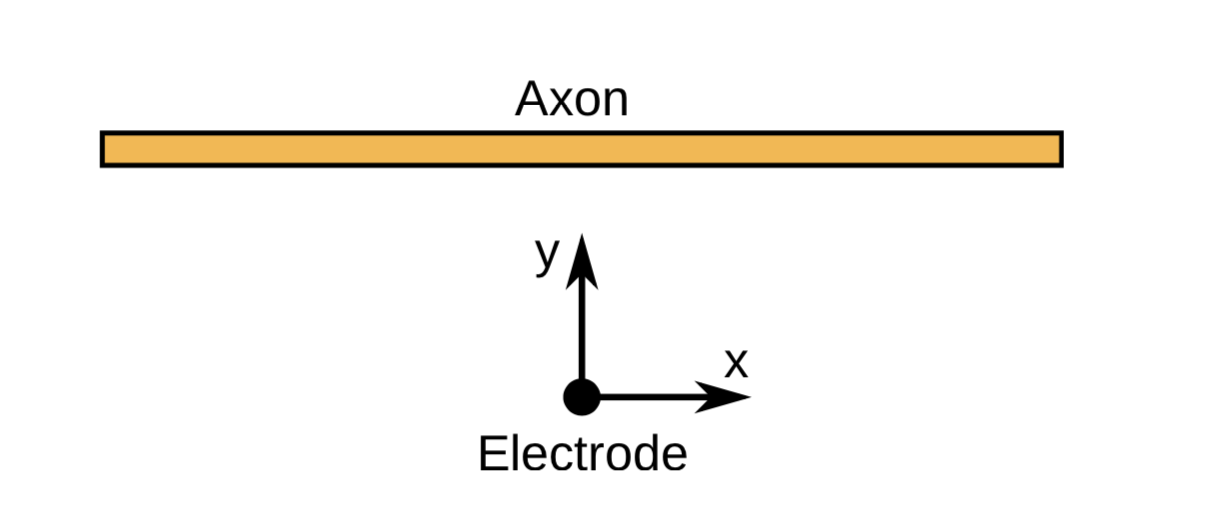
\includegraphics[width=.5\linewidth]{imgs/axon_img.png}
    \caption{Axon with current source.} 
    \label{fig:axon} 
\end{figure}

\begin{figure}[H] 
  \begin{subfigure}[b]{0.5\linewidth}
    \centering
    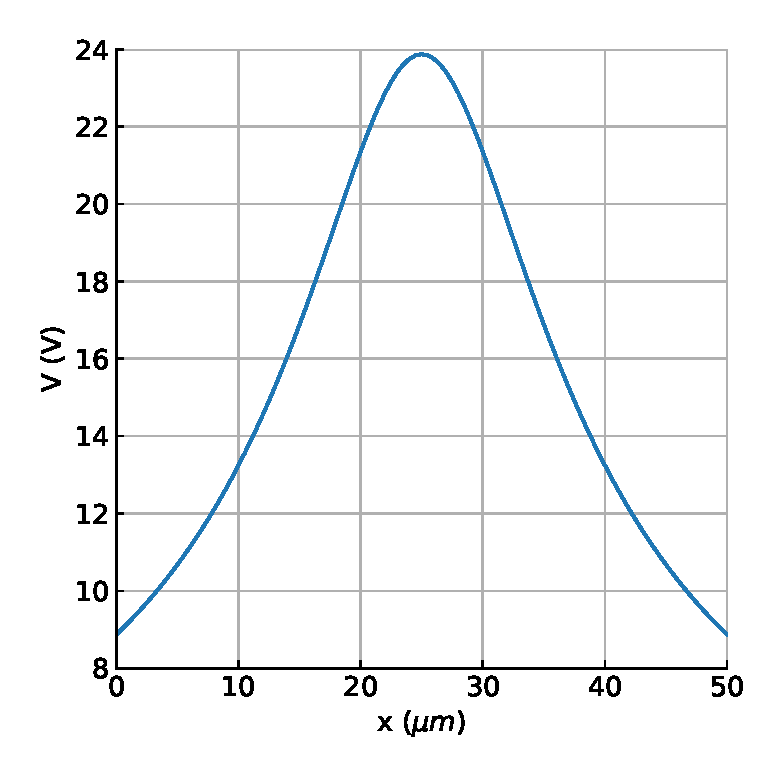
\includegraphics[width=\linewidth]{imgs/external_potential_0.eps} 
    \label{fig:ext0} 
  \end{subfigure}%% 
  \quad
  \begin{subfigure}[b]{0.5\linewidth}
    \centering
    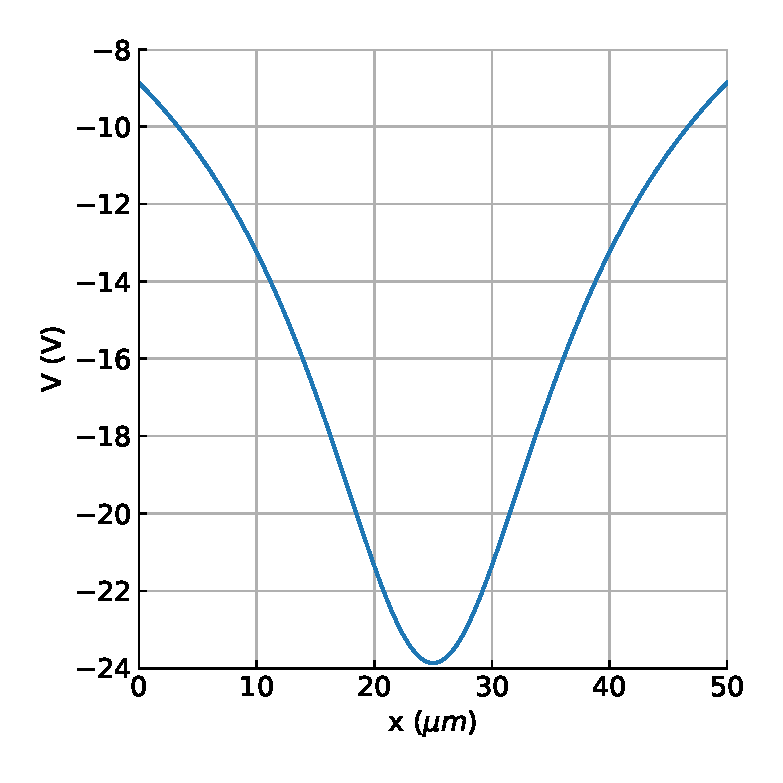
\includegraphics[width=\linewidth]{imgs/external_potential_1.eps} 
    \label{fig:ext1} 
    \end{subfigure} 
  \caption{External potential along an axon positioned at $\SI{10}{\micro\meter}$ from a current point source  plottet for different source currents. Left: $\SI{1}{\milli\ampere}$, right: $\SI{-1}{\milli\ampere}$.}
  \label{fig:istim} 
\end{figure}
\begin{figure}[H] 
  \begin{subfigure}[b]{0.5\linewidth}
    \centering
    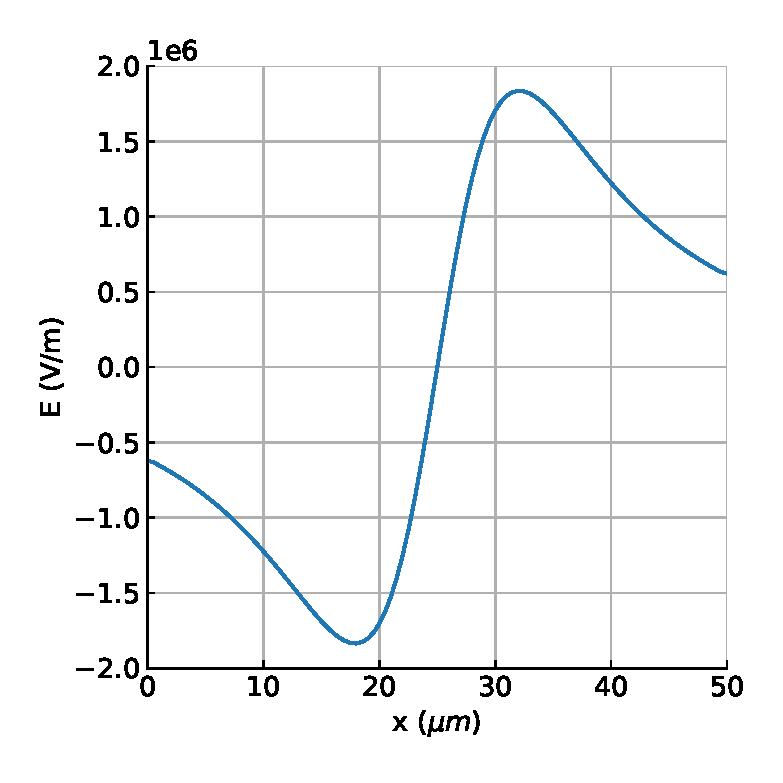
\includegraphics[width=\linewidth]{imgs/e_field_0.eps} 
    \label{fig:ext0} 
  \end{subfigure}%% 
  \quad
  \begin{subfigure}[b]{0.5\linewidth}
    \centering
    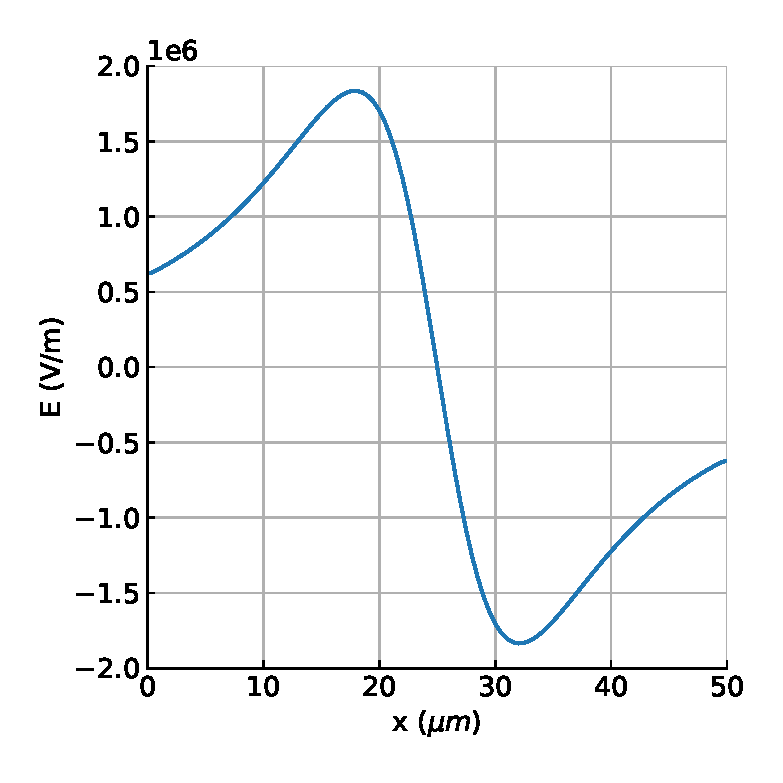
\includegraphics[width=\linewidth]{imgs/e_field_1.eps} 
    \label{fig:ext1} 
    \end{subfigure} 
  \caption{Electric field along an axon positioned at $\SI{10}{\micro\meter}$ from a current point source  plottet for different source currents. Left: $\SI{1}{\milli\ampere}$, right: $\SI{-1}{\milli\ampere}$.}
  \label{fig:istim} 
\end{figure}
\begin{figure}[H] 
  \begin{subfigure}[b]{0.5\linewidth}
    \centering
    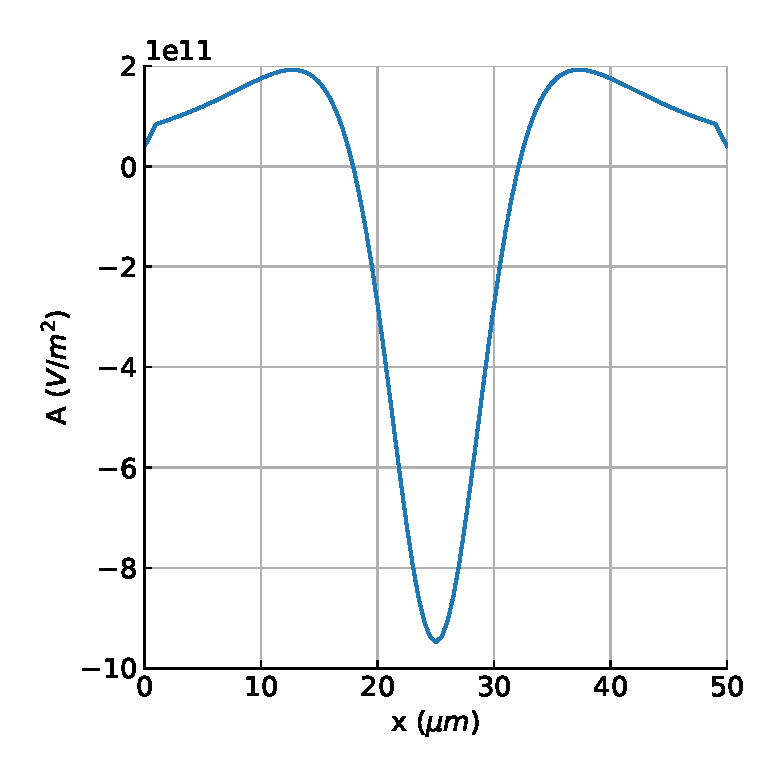
\includegraphics[width=\linewidth]{imgs/activation_0.eps} 
    \label{fig:ext0} 
  \end{subfigure}%% 
  \quad
  \begin{subfigure}[b]{0.5\linewidth}
    \centering
    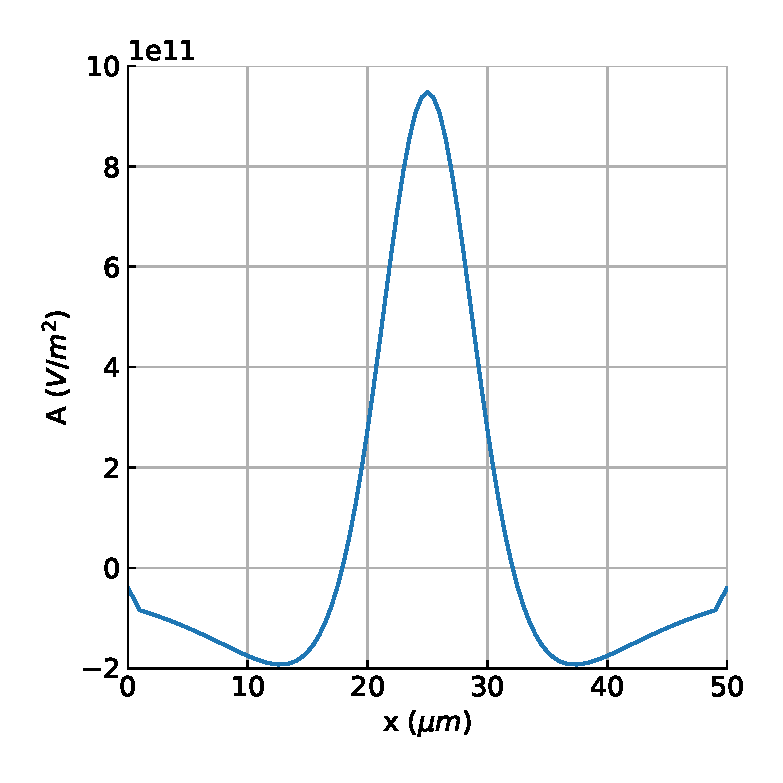
\includegraphics[width=\linewidth]{imgs/activation_1.eps} 
    \label{fig:ext1} 
    \end{subfigure} 
  \caption{Actionpotential along an axon positioned at $\SI{10}{\micro\meter}$ from a current point source  plottet for different source currents. Left: $\SI{1}{\milli\ampere}$, right: $\SI{-1}{\milli\ampere}$.}
  \label{fig:istim} 
\end{figure}

\section{Create a Neuron Model}

The model from the last exercise has been inhanced in order to consider the influence of an external potential. The parameters have been changed accordingly:
\begin{itemize}
\item $\rho_{axon} = \SI{0.01}{\kilo\ohm}\text{cm}$
\item $r_{axon} = \num{1.5e-4}$ cm
\item $l_{comp} = \num{0.5e-4}$ cm
\end{itemize}
The code written to generate the following plots can be found under \texttt{code/exercise\_6.py} and \texttt{code/Neuroprosthetics/multicompartment\_model.py}.

\subsection{Stimulate the Axon}
Create the following stimulation sequences and run a simulation with your axon positioned as in section 1.2. Run the simulation for about $\SI{30}{\milli\second}$ and position your pulse at $t = \SI{5}{\milli\second}$. Note that in these simulations there is no injected current $I_{stim}$. Any stimulation of the model originates from the external potential.
Do not forget that in the HH model we use $\SI{}{\milli\volt}$ for the potential.

\begin{enumerate}
\item Stimulation by a mono-phasic current pulse, phase duration = 1ms, current =
-0.25 mA
\item Stimulation by a mono-phasic current pulse, phase duration = 1ms, current =
−1 mA
\item Stimulation by a bi-phasic current pulse (negative phase first), phase duration =
1 ms, amplitude = 0.5 mA
\item Stimulation by a bi-phasic current pulse (negative phase first), phase duration =
1 ms, amplitude = 2 mA
\item Stimulation by a mono-phasic current pulse, phase duration = 1ms, current =
0.25 mA
\item Stimulation by a mono-phasic current pulse, phase duration = 1ms, current =
   5mA
\end{enumerate}

\subsection{Interpretation of the results}

In the experiments the Axon has been stimulated by an external electrode, positioned at $\SI{10}{\micro\meter}$ perpendicular distance from the center compartment  (Nr. 50) of the given axon piece.\\ Figure~\ref{fig:stim1} shows the axons reaction to an external stimulation induced by negative current pulses of  $\SI{-0.25}{\milli\ampere}$ and $\SI{-1}{\milli\ampere}$. The outcome for the former one can be seen in figure~\ref{fig:mm025mA}. The center most central compartments experience some little depolarization. However, this seems not to be enough to elicit an action potential. In the latter case instead concidering figure~\ref{fig:mm1mA}, it is apparent that the external stimmulation is sufficiently large for the center compartments to fire an action potential, which is them propagated along both sides of the axon.\\ Figure~\ref{fig:stim_bi} shows two cases for the external axon stimulation with a bi-phasic pulse. Like in figure~\ref{fig:stim1} stimulation with a smaller current, visible in figure~\ref{fig:bi05mA} charges the center compartments but does not suffice to provoke an action potential. Since with the bi-phasic current pulse the axon is stimmulated with a second - this time positive - pulse right after the depolarisation, the center compartments membrane potential returns to the resting potential faster than it was the case for the mono-phasic pulse in figure~\ref{fig:mm025mA}. The stimulation with $\SI{2}{\milli\ampere}$ in figure~\ref{fig:bi2mA}instead is comparable to figure~\ref{fig:mm1mA} only that due to the higher pulse amplitude, more of the centermost compartments are stimulated simultaniously.\\ 
Lastly, figure~\ref{fig:stim2} shows two different stimulations with positive mono-phasic current pulses. In figure~\ref{fig:m025mA} only a amall positive pulse of $\SI{0.25}{\milli\ampere}$ is applied by the electrode. Here, the center compartments near to the electrode are hyperpolarized, while compartments further away are being depolarized. The central compartments are then slightly depolarised with a timedelay of about $\SI{5}{\milli\second}$. Figure~\ref{fig:m5mA} instead shows the result of a stimulation with $\SI{5}{\milli\ampere}$. In this case, compartments further away from the electrode are depolarized enough to elicit an action potential right away, and pass this on to both sides of the axon. Only after around $\SI{10}{\milli\second}$ the centermost compartments are depolarized and elicit an action potential, too. Because of the compartments absolute refractory period the action potential coming from the more proximal and the more distal part of the axon are no further propagated ones they coincide with the action potential propagated from the center compartments at $t=\SI{25}{\milli\second}$.

\begin{figure}[H] 
  \begin{subfigure}[b]{\linewidth}
    \centering
    \includegraphics[width=\linewidth]{imgs/model_monophasic_m025.eps}
    \caption{Pulse amplitude: $\SI{-0.25}{\milli\ampere}$.} 
    \label{fig:mm025mA} 
  \end{subfigure}%% 
  \quad
  \begin{subfigure}[b]{\linewidth}
    \centering
    \includegraphics[width=\linewidth]{imgs/model_monophasic_m1.eps} 
    \caption{Pulse amplitude: $\SI{-1}{\milli\ampere}$.}
    \label{fig:mm1mA} 
    \end{subfigure} 
  \caption{Propagation of the action potential when stimulated at $t = \SI{5}{\milli\second}$ with a negative mono-phasic pulse and a phase duration of $\SI{1}{\milli\second}$.}
  \label{fig:stim1} 
\end{figure}

\begin{figure}[H] 
	\begin{subfigure}[b]{\linewidth}
    \centering
    \includegraphics[width=\linewidth]{imgs/model_biphasic_05.eps}
    \caption{Pulse amplitude: $\SI{0.5}{\milli\ampere}$.}
    \label{fig:bi05mA} 
    \end{subfigure} %%
    \quad
  \begin{subfigure}[b]{\linewidth}
    \centering
    \includegraphics[width=\linewidth]{imgs/model_biphasic_2.eps} 
    \caption{Pulse amplitude: $\SI{2}{\milli\ampere}$.}
    \label{fig:bi2mA} 
  \end{subfigure}
  \caption{Propagation of the action potential when stimulated at $t = \SI{5}{\milli\second}$ with a bi-phasic pulse (negative phase first) and a phase duration of $\SI{1}{\milli\second}$.}
  \label{fig:stim_bi}
\end{figure}

\begin{figure}[H] 
  \begin{subfigure}[b]{\linewidth}
    \centering
    \includegraphics[width=\linewidth]{imgs/model_monophasic_025.eps} 
    \caption{Pulse amplitude: $\SI{0.25}{\milli\ampere}$.}
    \label{fig:m025mA} 
    \end{subfigure} %%
    \quad 
    \begin{subfigure}[b]{\linewidth}
    \centering
    \includegraphics[width=\linewidth]{imgs/model_monophasic_5.eps} 
    \caption{Pulse amplitude: $\SI{5}{\milli\ampere}$.}
    \label{fig:m5mA} 
    \end{subfigure} 
  \caption{Propagation of the action potential when stimulated at $t = \SI{5}{\milli\second}$ with a positive mono-phasic pulse and a phase duration of $\SI{1}{\milli\second}$.}
  \label{fig:stim2} 
\end{figure}


\end{document}
